\chapter{Probabilistic Graphical Models}
\label{chap: probabilistic graphical models}


\section{Directed Graphical Models}

\subsection{Dynamical Latent Variable Models}
\label{sec: dynamical latent variable models}

To model a sequence of $T$ observations, $\mathbf{x}_{1:T}$, one can use a dynamical latent variable model, $p_\theta (\mathbf{x}_{1:T}, \mathbf{z}_{1:T})$, which models the joint distribution between $\mathbf{x}_{1:T}$ and a sequence of latent variables, $\mathbf{z}_{1:T}$, with parameters $\theta$. Using a directed graphical model, $p_\theta (\mathbf{x}_{1:T}, \mathbf{z}_{1:T})$ can be factorized into conditional joint distributions, $p_\theta (\mathbf{x}_t, \mathbf{z}_t | \mathbf{x}_{1:t-1}, \mathbf{z}_{1:t-1})$, at each time step $t$, which are conditioned on all preceding variables:
\begin{equation}
    p_\theta (\mathbf{x}_{1:T}, \mathbf{z}_{1:T}) = \prod_{t=1}^T p_\theta (\mathbf{x}_t, \mathbf{z}_t | \mathbf{x}_{1:t-1}, \mathbf{z}_{1:t-1}) = \prod_{t=1}^T p_\theta (\mathbf{x}_t | \mathbf{x}_{1:t-1}, \mathbf{z}_{1:t}) p_\theta (\mathbf{z}_t | \mathbf{x}_{1:t-1}, \mathbf{z}_{1:t-1}).
    \label{eq: general dynamics model}
\end{equation}
A plate notation diagram for the full graphical model is shown in Figure \ref{fig: full_dynamical_model}. The distribution $p_\theta (\mathbf{x}_t | \mathbf{x}_{1:t-1}, \mathbf{z}_{1:t})$ is commonly referred to as the observation or measurement model, and $p_\theta (\mathbf{z}_t | \mathbf{x}_{1:t-1}, \mathbf{z}_{1:t-1})$ is the dynamics or transition model. Conditioning through a direct functional dependence on all past variables requires a method of storing and accessing this information, which becomes intractable, in terms of both memory and computation, as the sequence length grows. To overcome this intractability, the model is typically assumed to be Markovian, meaning that
\begin{itemize}
    \item the states form a Markov sequence, $p_\theta (\mathbf{z}_t | \mathbf{x}_{1:t-1}, \mathbf{z}_{1:t-1}) = p_\theta (\mathbf{z}_t | \mathbf{z}_{t-1}) $, and
    \item the observations are conditionally independent of all other latent variables and observations given the current latent variable, $p_\theta (\mathbf{x}_t | \mathbf{x}_{1:t-1}, \mathbf{z}_{1:t}) = p_\theta (\mathbf{x}_t | \mathbf{z}_t)$.
\end{itemize}
In other words, it is assumed that the latent variable at a particular time step contains all of the information necessary to summarize the corresponding observation and all future and past latent variables. Eq. \ref{eq: general dynamics model} then becomes:
\begin{equation}
    p_\theta (\mathbf{x}_{1:T}, \mathbf{z}_{1:T}) = \prod_{t=1}^T p_\theta (\mathbf{x}_t, \mathbf{z}_t | \mathbf{z}_{t-1}) = \prod_{t=1}^T p_\theta (\mathbf{x}_t | \mathbf{z}_{t}) p_\theta (\mathbf{z}_t | \mathbf{z}_{t-1}).
    \label{eq: markov dynamics model}
\end{equation}
A plate notation diagram for the updated model is shown in Figure \ref{fig: markov_dynamical_model}.

\begin{figure*}[t!]
    \centering
    \begin{subfigure}[t]{0.5\textwidth}
        \centering
        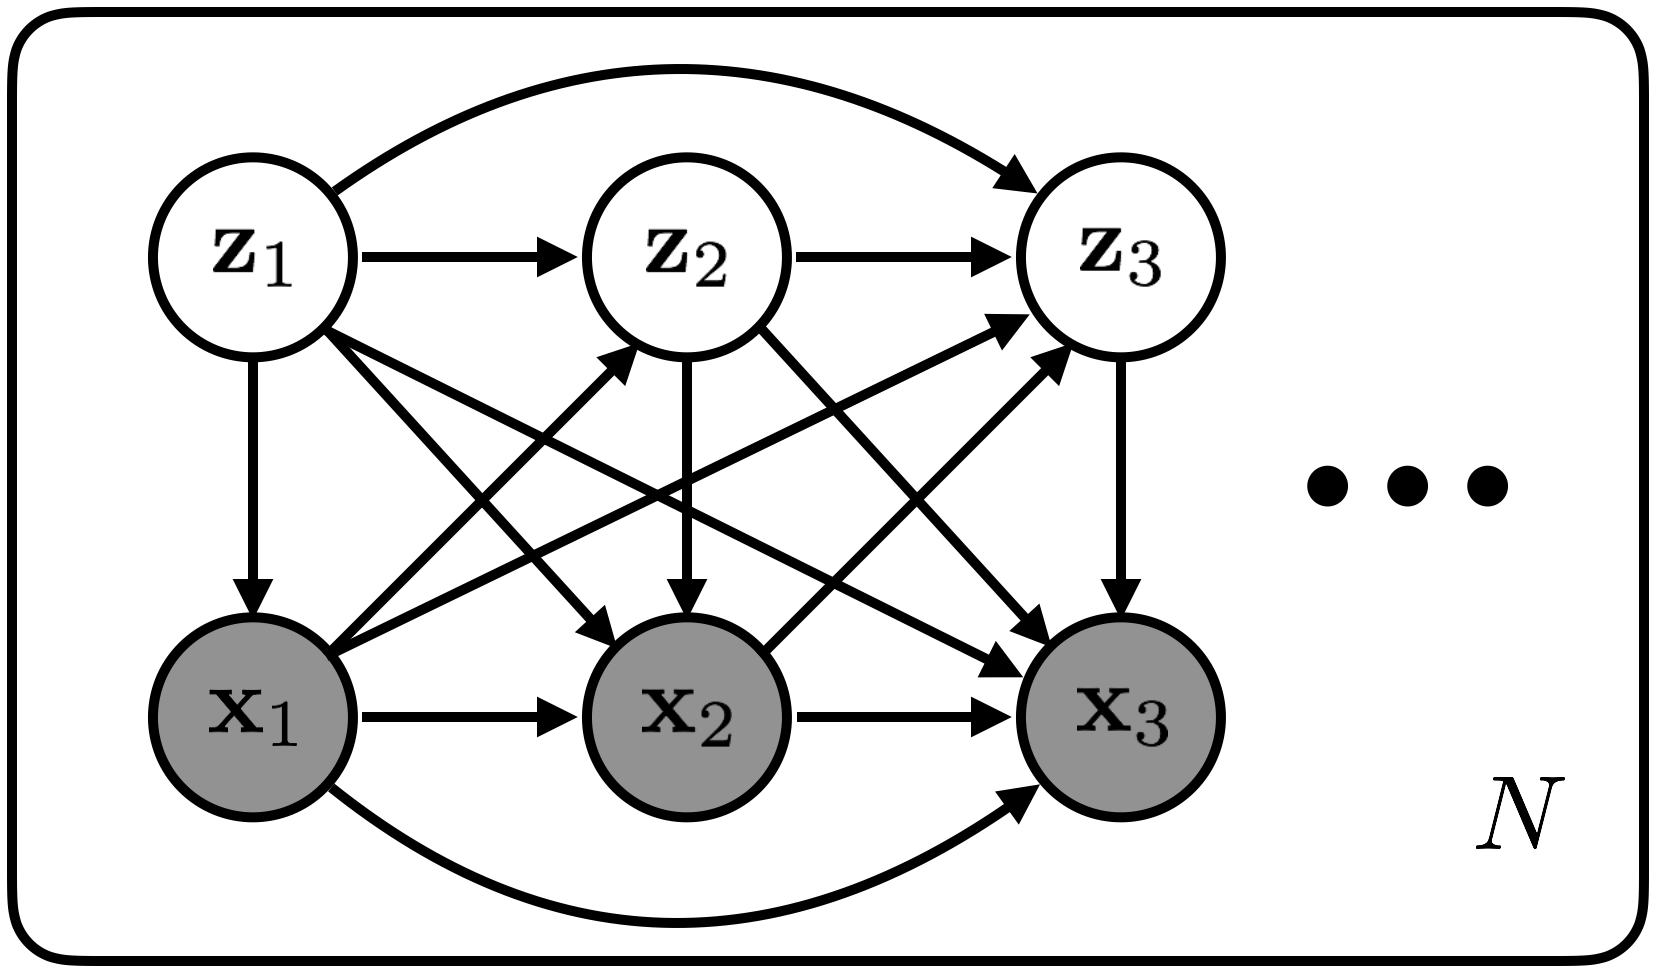
\includegraphics[width=0.8\textwidth]{images/graphical_models/full_dynamical_model.png}
        \caption{ }
        \label{fig: full_dynamical_model}
    \end{subfigure}%
    ~ 
    \begin{subfigure}[t]{0.5\textwidth}
        \centering
        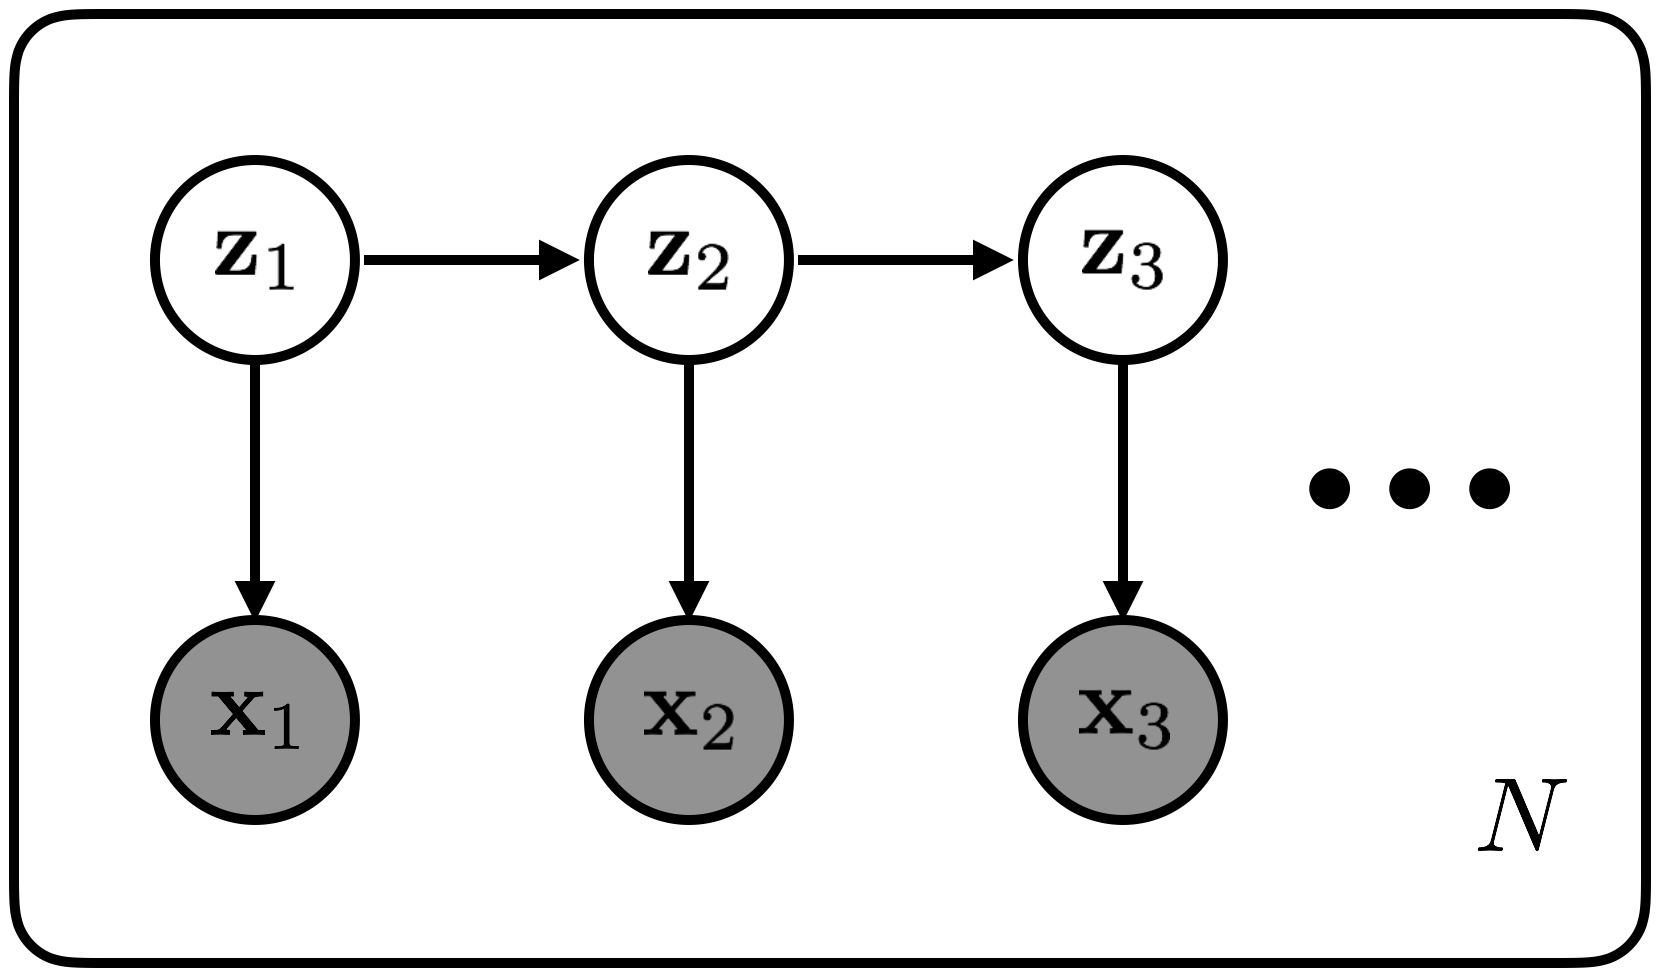
\includegraphics[width=0.8\textwidth]{images/graphical_models/markov_dynamical_model.png}
        \caption{ }
        \label{fig: markov_dynamical_model}
    \end{subfigure}
    \caption{Plate notation diagrams for dynamical latent variable models with (a) all temporal dependencies and (b) the Markov assumption. Plates denote that there are $N$ example sequences. Parameters $\theta$ have been omitted for clarity.}
\end{figure*}

\subsubsection{Bayesian Filtering}

Dynamical directed latent variable models naturally lend themselves to a \textit{filtering} setting \cite{sarkka2013bayesian}, in which one computes the marginal posterior distribution, $p(\mathbf{z}_t | \mathbf{x}_{1:t})$, at each time step. This corresponds to estimating the current state of the system given all past observations. Under the Markov assumption (eq. \ref{eq: markov dynamics model}), we start with a latent prior, $p_\theta (\mathbf{z}_1)$, and compute the marginal posterior at some time step $t$ by recursively applying the following steps:
\begin{enumerate}
	\item \textbf{Prediction}: use the Chapman-Kolmogorov equation to form a prior (i.e. prediction) on the latent variable at the next time step: 
\begin{equation}
	p(\mathbf{z}_t | \mathbf{x}_{1:t-1}) = \int p_\theta (\mathbf{z}_t | \mathbf{z}_{t-1}) p_\theta (\mathbf{z}_{t-1} | \mathbf{x}_{1:t-1}) d\mathbf{z}_{t-1}.
\end{equation}
	\item \textbf{Update}: use the prediction, along with Bayes' rule, to update the marginal posterior:
\begin{equation}
	p(\mathbf{z}_t | \mathbf{x}_{1:t}) = \frac{p_\theta (\mathbf{x}_t | \mathbf{z}_t) p_\theta (\mathbf{z}_t | \mathbf{x}_{1:t-1})}{p_\theta (\mathbf{x}_{1:t})},
\end{equation}
	where $p_\theta (\mathbf{x}_{1:t})$ is calculated as
\begin{equation}
	p_\theta (\mathbf{x}_{1:t}) = \int p_\theta (\mathbf{x}_t | \mathbf{z}_t) p_\theta (\mathbf{z}_t | \mathbf{x}_{1:t-1}) d\mathbf{z}_t.
\end{equation}
\end{enumerate}
When $p_\theta (\mathbf{x}_t | \mathbf{z}_t)$ and $p_\theta (\mathbf{z}_t | \mathbf{x}_{1:t-1})$ are parameterized as linear functions that take a Gaussian form, the resulting model is referred to as a Kalman filter \cite{kalman1961new}. However, in general, the prediction and update steps are both intractable, as they involve integrating over the space of latent variables. To overcome these intractabilities, one must turn to forms of approximate inference (see Section \ref{sec: variational inference in dynamical models}).

% The joint prior distribution of the states is given as:
% \begin{equation}
% 	p(z_{0:T}) = p(z_0) \prod_{t=1}^T p(z_t | z_{t-1}).
% \end{equation}
% The joint conditional likelihood of measurements is given as:
% \begin{equation}
% 	p(x_{1:T} | z_{0:T}) = \prod_{t=1}^T p(x_t | z_t).
% \end{equation}
% The full posterior (which is intractable) is given as:
% \begin{equation}
%	p(z_{0:T} | x_{1:T}) = \frac{p(x_{1:T} | z_{0:T}) p(z_{0:T})}{p(x_{1:T})}.
% \end{equation}

\subsubsection{Beyond the Markov Assumption}
While drastically simplifying the model, the Markov assumption is often invalid in practical settings, where one commonly encounters partial observations (i.e. hidden information) or correlated observation noise across time. In such cases, the ``memoryless" or ``static world" properties of the Markov assumption no longer hold, requiring that we expand the model to condition on past variables. This can be accomplished through
\begin{itemize}
	\item conditioning on a concatenation of variables containing the recent trajectory,
	\item memory mechanisms that selectively store state information \cite{chung2015recurrent, fraccaro2016sequential, gemici2017generative},
	\item modeling the observations and latent variables in generalized coordinates \cite{friston2010generalised}.
\end{itemize}

\section{Undirected Graphical Models}
\label{sec: undirected models}


\section{Causal Models}
\label{sec: causal models}

\subsection{Observational vs. Interventional Distributions}

This section is based on a blog post by Ferenc Husz\'ar\footnote{\texttt{http://www.inference.vc/untitled/}}. Say we have a joint probability distribution $p(x, y, z, \dots)$. Often, we are interested in conditional probabilities, for instance, how $y$ behaves given $x$. There are, in fact, two forms of this probability:
\begin{itemize}
    \item \textbf{Observational} $p(y | x)$: this is the probability of $Y = y$ given that I \textit{observe} $X = x$. This is the typical use of conditional probability in machine learning, where we simply use Bayes rule to marginalize over the joint distribution, i.e. $p(y | x) = \frac{p(y, x)}{p(x)}$.
    \item \textbf{Interventional} $p(y | do(x))$: this is the probability of $Y=y$ given that I \textit{set} $X=x$. Here, we are intervening in the data generating process. Note that the data generating process is not the same as the joint distribution.
\end{itemize}
The observational and interventional conditional probabilities are not generally the same. Ferenc gives the simple example of a sensor monitoring the value of a given quantity, such as pressure. Observing the sensor reading allows one to infer the pressure. However, intervening to change the reading on the sensor will have no effect on the pressure. Hence, $p(y|x)$ and $p(y|do(x))$ are quite different. The first simply describes statistical relationships, whereas the second describes the second describes causal relationships. The observational conditional is often sufficient for many machine learning applications, but when dealing with tasks related to decision making or control, the interventional conditional is typically more useful.

Like the observational conditional, the interventional conditional distribution, $p(y | do(x))$, is just a probability distribution that we can calculate using Bayes rule. The difference is that $p(y | do(x))$ is calculated from a separate \textit{interventional joint distribution}, $$p_{do(X=x)} (x, y, z, \dots).$$
\noindent This is the joint distribution of the variables when we conduct randomized control experiments by intervening in the data generating process to set $X=x$. Even if it is impossible or unethical to conduct these intervention experiments, this joint distribution exists. One of the main points of causal modeling is estimating the interventional conditional when we only have observations.

\begin{figure}[t!]
    \centering
    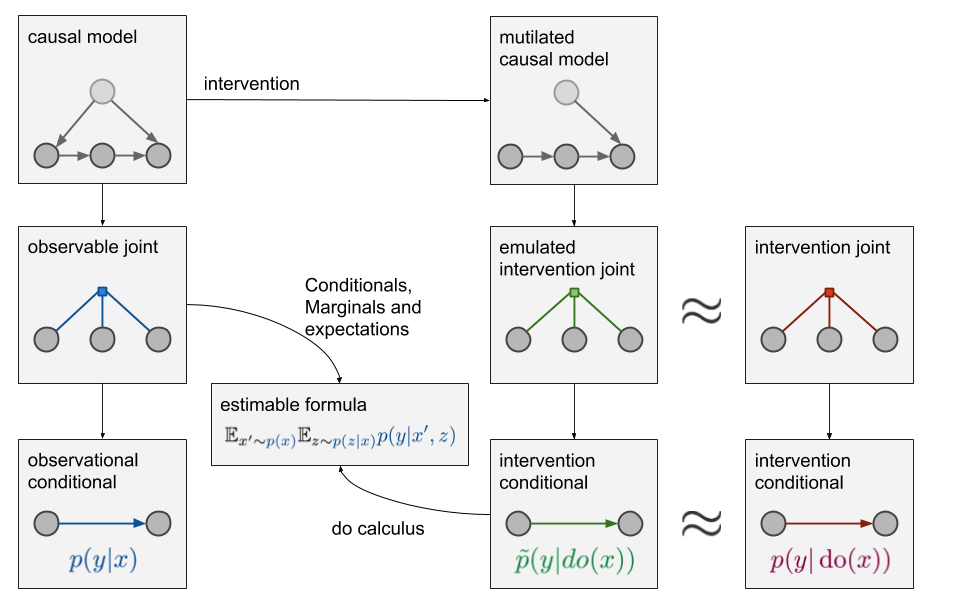
\includegraphics[width=0.8\textwidth]{images/graphical_models/Causality_-do-calculus-estimand--1-.png}
    \caption{Pipeline of causal modeling with do-calculus. Often, we only have access to the observational joint distribution, $p(x, y, z, \dots)$ but want to estimate the interventional conditional $p(y | do(x))$. To do so, we must assume a causal model and use do-calculus to arrive at an estimated interventional conditional $\tilde{p}(y | do(x))$. Note that this may not always be feasible. Reproduced from \texttt{http://www.inference.vc/untitled/}.}
    \label{fig: causal_model}
\end{figure}

\subsection{Causal Modeling \& Do-Calculus}

Supervised learning is a great technique for estimating conditional distributions. Given a joint distribution of random variables, it is fairly straightforward to train a model to estimate the conditionals. This is true of both observational and interventional conditionals, assuming one has access to the appropriate joint distribution. Recall, however, that in many cases the joint distribution contains observations rather than interventions. How, then, can we estimate the interventional conditional if we don't have direct access to the interventional joint distribution? Doing this requires making further assumptions about the structure of the data generating process. That is, we must assume a \textit{causal model} of the data, which provides information that is not captured by the observational joint distribution alone. Arrows in causal models represent direct causal directions, while the absence of an arrow denotes a lack of direct casual influence.

To estimate the interventional conditional distribution using the observational joint, one must ``mutilate" the assumed causal model to emulate the desired intervention. One then uses \textit{do-calculus} to attempt to estimate $p(y | do(x))$ from the conditionals and marginals of the observational joint distribution, yielding $\tilde{p}(y | do(x))$. Importantly, this approximation may or may not be \textit{identifiable}, depending on whether other variables in the joint distribution are observed. This pipeline is shown in Figure \ref{fig: causal_model}.


\section{Transformation of Variables}
\label{sec: transformation of variables}

Real-valued non-volume preserving (Real NVP) transformations provide a tractable method of performing learning and inference in a non-linear latent variable model \cite{dinh2016density}. With a bijective generative mapping $g$, latent variable $\mathbf{z} \sim p_z (\mathbf{z})$, and observation $\mathbf{x} \sim p_x (\mathbf{x})$, the density over observations can be modeled using the transformation of variables formula:
\begin{equation}
	p_x (\mathbf{x}) = p_z (\mathbf{z}) \bigg \vert \text{det} \left( \frac{\partial g(\mathbf{z})}{\partial \mathbf{z}^T} \right) \bigg \vert^{-1}.
	\label{eq: real nvp transform of variables 1}
\end{equation}
Using the bijection $f = g^{-1}$, equation \ref{eq: real nvp transform of variables 1} can also be written as
\begin{equation}
	p_x (\mathbf{x}) = p_z (f(\mathbf{x})) \bigg \vert \text{det} \left( \frac{\partial f(\mathbf{x})}{\partial \mathbf{x}^T} \right) \bigg \vert 
	\label{eq: real nvp transform of variables 2}
\end{equation}
\begin{equation}
	\log \left( p_x (\mathbf{x}) \right) = \log \left( p_z (f(\mathbf{x})) \right)  + \log \left( \bigg \vert \text{det} \left( \frac{\partial f(\mathbf{x})}{\partial \mathbf{x}^T} \right) \bigg \vert \right).
	\label{eq: real nvp transform of variables 3}
\end{equation}
Because the mapping between $\mathbf{x}$ and $\mathbf{z}$ is invertible, we can perform exact inference and evaluation with the model. Also note that evaluation of the log-likelihood, $\log \left( p_x (\mathbf{x}) \right)$, does not require a fixed-form reconstruction cost, such as $L^2$ distance, because the terms on the right side of eq. \ref{eq: real nvp transform of variables 3} can be computed using the data, mapping, and prior. Inference and generation procedures are shown for a simple two dimensional example in Figure \ref{fig: transform of variables}.
\begin{figure}[h]
    \centering
    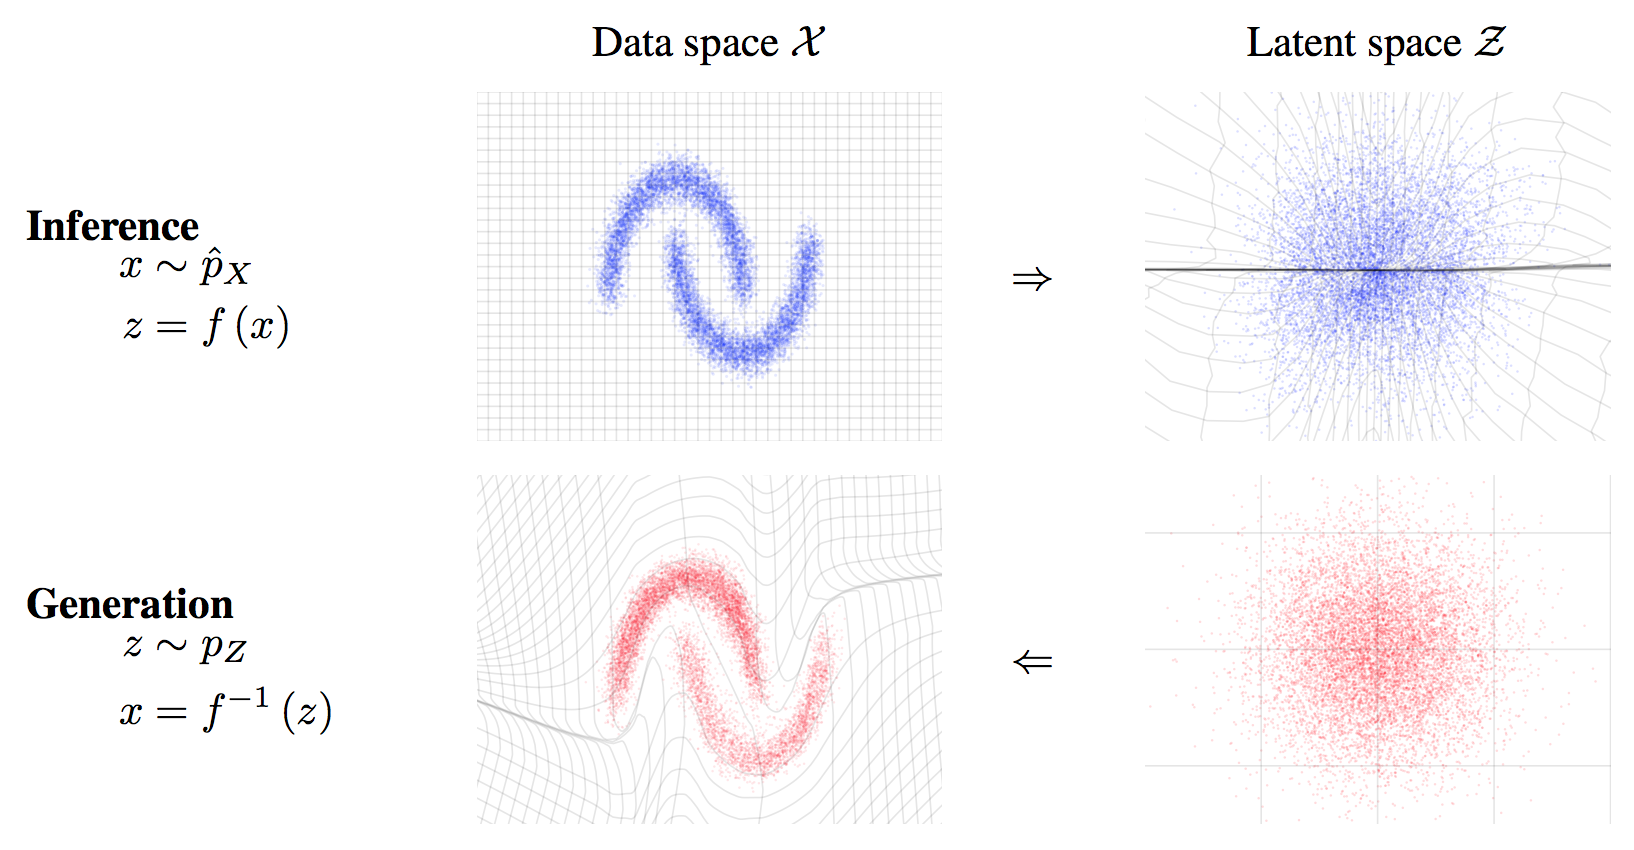
\includegraphics[width=0.8\textwidth]{images/graphical_models/transform_of_variables.png}
    \caption{Inference and generation through transformation of variables in 2D. The invertible mapping between the observed and latent variables warps the respective spaces. Reproduced from \cite{dinh2016density}.}
    \label{fig: transform of variables}
\end{figure}

In general, computing eq. \ref{eq: real nvp transform of variables 3} is intractable for high-dimensional variables, stemming from computing the log determinant of the Jacobian matrix. However, by carefully designing the mapping, we can achieve a lower triangular Jacobian matrix, the determinant of which is simply the product of the diagonal elements. Given a $D$ dimensional input $\mathbf{x}$ and $d < D$, an \textit{affine coupling layer} with output $\mathbf{y}$ is defined as 
\begin{align}
	\mathbf{y}_{1:d} &= \mathbf{x}_{1:d},
	\label{eq: real nvp mapping 1} \\
	\mathbf{y}_{d+1:D} &= \mathbf{x}_{d+1:D} \odot \exp (s(\mathbf{x}_{1:d})) + t(\mathbf{x}_{1:d}),
	\label{eq: real nvp mapping 2}
\end{align}
where $s(\mathbf{x}_{1:d})$ and $t(\mathbf{x}_{1:d})$ are respectively \textit{scale} and \textit{translation} functions from $\mathbb{R}^d \rightarrow \mathbb{R}^{D-d}$. The Jacobian of this transformation is
\begin{equation}
	\frac{\partial \mathbf{y}}{\partial \mathbf{x}^T} =
	\begin{bmatrix}
    \mathbf{I}_d & 0 \\
    \frac{\partial \mathbf{y}_{d+1:D}}{\partial \mathbf{x}^T_{1:d}}  & \text{diag} \left( \exp \left( s(\mathbf{x}_{1:d}) \right) \right)
\end{bmatrix}.
\end{equation}
Therefore, the determinant of the Jacobian can be easily computed as
\begin{equation}
	\text{det} \left( \frac{\partial \mathbf{y}}{\partial \mathbf{x}^T}  \right) = \exp \left( \sum_j s(\mathbf{x}_{1:d})_j \right).
\end{equation}
Note that $s$ and $t$ can be any arbitrary functions, as only their output values enter into inference and evaluation. Furthermore, the mapping in eqs. \ref{eq: real nvp mapping 1} and \ref{eq: real nvp mapping 2} can be inverted without computing the inverse of $s$ or $t$:
\begin{align}
	\mathbf{x}_{1:d} &= \mathbf{y}_{1:d}, \\
	\mathbf{x}_{d+1:D} &= (\mathbf{y}_{d+1:D} - t(\mathbf{x}_{1:d})) \odot \exp (- s(\mathbf{x}_{1:d})).
\end{align}
By composing multiple coupling layers, one can construct more expressive transformations. Successive coupling layers alternate between transforming different subsets of the input dimensions. The determinants of the Jacobians, as well as the inverse mappings, can still be computed easily. The authors of \cite{dinh2016density} use checkerboard and channel-wise masked convolutional networks to implement $s$ and $t$, with a hierarchy of resolutions. Other possible transformations are possible instead of coupling layers, such as normalizing and inverse auto-regressive flow.

NICE: \cite{dinh2014nice}







